\section{Тестирование}

\begin{frame}
\frametitle{Тестирование}
\begin{columns}[T]
\begin{column}{0.30\textwidth}
Модуль анализа позволяет построить графики и таблицы по заданному фильтру.

\vspace{1.5cm}

Рейтинг ресурсов:
\begin{tabular}{|l|l|}
\hline
Имя ресурса & Переходы\\
\hline
сайт 1 & $n_1$\\
\hline
\dots & \\
\hline
сайт i & $n_i$\\
\hline
\dots & \\
\hline
сайт $N$ & $n_{N}$\\
\hline
\end{tabular}
\end{column}
\begin{column}{0.70\textwidth}
\vspace{0.2cm}
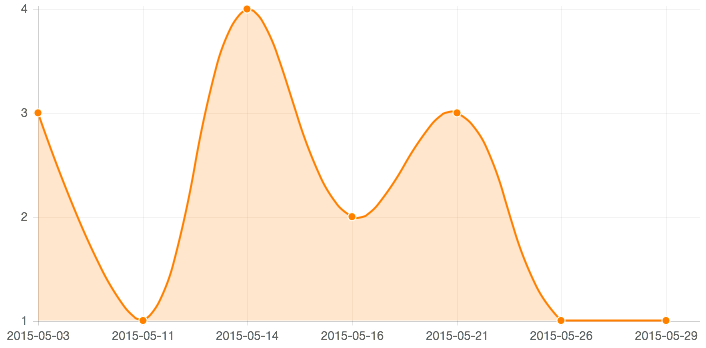
\includegraphics[width=0.95\textwidth]{images/chart}

\hspace{1cm} $n_i$ --- количество переходов с сайта $i$

\hspace{1cm} $n_1 \geq n_i \geq n_{N}$


\hspace{1cm} По оси абсцисс отмечаются $d \in D$

\hspace{1cm} По оси ординат отмечаются $\sum\limits_{i \in I, r \in R} x (r,i,d)$

\end{column}
\end{columns}
\end{frame}

